\documentclass[11pt,a4paper]{article}

\usepackage[a4paper,hmargin=2.5cm,vmargin=2.3cm]{geometry}
\usepackage[T1]{fontenc}
\usepackage{amsmath}
\usepackage{amsthm}
\usepackage{newtxtext}
\usepackage{newtxmath}
\usepackage{microtype}
\usepackage{booktabs}
\usepackage{graphicx}
\usepackage{array}
\usepackage{tabularx}
\usepackage{longtable}
\usepackage[font=small,labelsep=period,skip=4pt]{caption}
\usepackage[numbers,sort&compress]{natbib}
\usepackage{titlesec}
\usepackage{enumitem}
\usepackage{xurl}
\usepackage[colorlinks=true,allcolors=black]{hyperref}

\titleformat{\section}{\normalfont\large\scshape\centering}{\thesection.}{0.5em}{}
\titleformat{\subsection}{\normalfont\itshape}{\thesubsection}{0.5em}{}
\titlespacing*{\section}{0pt}{2.0ex plus 0.5ex}{1.0ex}
\titlespacing*{\subsection}{0pt}{1.4ex plus 0.4ex}{0.5ex}
\setlist[enumerate]{label=\arabic*.,leftmargin=2.0em,itemsep=0.1ex,topsep=0.4ex}
\theoremstyle{definition}
\newtheorem*{definition}{Definition}
\renewcommand{\figurename}{Fig.}
\setlength{\tabcolsep}{4pt}
\setlength{\textfloatsep}{12pt plus 2pt minus 2pt}

\renewcommand{\bibfont}{\small}
\setlength{\bibsep}{2pt plus 1pt}
\newcommand{\dfresh}{\Delta_{\mathrm{fresh}}}
\newcommand{\KS}{$K\!-\!S$}
\newcommand{\tulu}{\textit{tulu}}
\newcommand{\smoltalk}{\textit{smoltalk}}
\newcommand{\mathcot}{\textit{mathcot}}
\newcommand{\pp}{\,pp}

\hypersetup{pdftitle={The Code Length of Post-Trained Language Models on Fresh Text},pdfauthor={Musaab Mahjoub}}

\title{\vspace{-1.6cm}The Code Length of Post-Trained Language Models on Fresh Text}
\author{Musaab Mahjoub\\[0.3ex]\normalsize Independent researcher}
\date{October 2026}

\begin{document}
\maketitle

\begin{abstract}
\noindent We evaluate a known quantity as a meter of what post-training costs: the increase over the base model
of a post-trained model's code length, its cross-entropy in bits per byte, on text first published or scanned
after the models were released, measured for 12 public post-trained checkpoints of 0.5 to 3 billion parameters
and for 12 checkpoints of our own fine-tuning runs. Post-training increased the code length in every comparison,
by about 0.1\% for pure reinforcement learning and up to 43\% for mathematical continued pretraining followed by
reasoning distillation, and one temperature removed at most 35\% of the increase. Across the public checkpoints
the increase went with the instruction-following gain and, above 15\%, with lost zero-shot accuracy, both
readings made after the data were seen. Within one base and three recipes it tracked neither: the one recipe that
lost accuracy lost about 4\% from the first checkpoint evaluated, all of it on ARC, and whether answer format
explains that loss is still under test.
\end{abstract}

\section{Introduction}

The entropy of a language can be estimated from the number of bits a good predictor needs to encode its text
\citep{shannon1948,shannon1951,cover1978}. A language model is such a predictor, and its code length on unseen
text has been proposed as a measure of what it has learned \citep{deletang2024compression,huang2024compression,
lotfi2024bounds}. Huang et al.\ \citep{huang2024compression} found, across 31 base models and 12 benchmarks, that
the average benchmark score is close to a linear function of the average bits per character on held-out text,
with a Pearson correlation of $-0.93$, and of about $-0.95$ within each domain. They excluded fine-tuned models, on
the ground that such a model no longer predicts arbitrary text but only structured query and response data.
Kalajdzievski \citep{kalajdzievski2024scaling} took the opposite view of the same quantity for fine-tuned models:
the cross-entropy to the base model's predictions on WikiText-103 served as the measure of forgetting itself.

In the present paper we test whether the increase in code length over the base is such a measure. We call the
relative increase the \emph{drift}; it is the relative increase in held-out negative log-likelihood, or in
log-perplexity, and the word is used in no other sense. Three questions are taken in order: how large the drift of
each post-training stage is; whether one temperature undoes it; and whether it predicts what post-training cost in
general benchmark accuracy while ignoring what it gained. The third is the practical one. The general benchmarks
of our suite take a median of 167\,s per checkpoint on an A10 GPU, and the drift a median of 15\,s on a T4, about
11 times less; in our own runs the drift took 5\,s on an A40 against 157 to 195\,s for the benchmarks on an A10,
30 to 37 times less.

The answers are the following.
\begin{enumerate}
\item Post-training increased the code length in all 15 comparisons: by 0.1--0.5\% for the three RL checkpoints,
1--7\% per step of supervised fine-tuning (SFT) or preference optimisation (DPO), and 16--43\% for distillation
and mathematical training (Section~\ref{sec:stages}). One temperature recovers at most 35\% of it
(Section~\ref{sec:temperature}).
\item Across the 12 public checkpoints the drift correlates with forgetting at $r=0.89$, but one lineage carries
the correlation (family-level interval $[-0.64,\,0.99]$). Read after the fact, the drift went with the
instruction-following gain ($r=0.89$) and, above 15\%, with forgetting. The absolute code length still ranks the
post-trained checkpoints by general score, $r=-0.81$ (Section~\ref{sec:benchmarks}).
\item Across token classes the drift is close to one-dimensional; a knowledge-minus-style contrast gave a lead
(Section~\ref{sec:classes}).
\item At equal drift on one base, neither the drift nor the contrast tracked forgetting or the gain. The forgetting
recipe lost about 4\% at every checkpoint, all of it on ARC, and the other two lost nothing on a six-task mean that
balances ARC losses against MMLU gains (Section~\ref{sec:matched}). A further experiment tests whether the ARC
losses are a matter of answer format, and the readings of Section~\ref{sec:discussion} are conditional on it.
\end{enumerate}
Four of the six experiments, on the staged checkpoints (Section~\ref{sec:stages}), the benchmarks
(Section~\ref{sec:benchmarks}), the token classes (Section~\ref{sec:classes}) and the controlled recipes
(Section~\ref{sec:matched}), were pre-registered: their rules and expected values were committed to the repository before
the runs, and Appendix~\ref{app:prereg} gives the commits and sets the rules beside the outcomes. The first
experiment, on the four laptop pairs of Section~\ref{sec:stages}, had no stated rule, and the rule of the temperature experiment was committed with its results. Every
reading added after a run is marked as such.

\section{Definitions}
\label{sec:definitions}

Let $x=x_1\cdots x_n$ be a text, encoded as tokens, and $q$ a language model with conditional probabilities
$q(x_i\mid x_{<i})$.

\begin{definition}
The \emph{code length} of $x$ under $q$ is $L_q(x)=-\sum_{i}\log_2 q(x_i\mid x_{<i})$, in bits: the negative
log-likelihood in base 2. Divided by the number of UTF-8 bytes of $x$ it is the cross-entropy in bits per byte
(bpb).
\end{definition}

\noindent For example, Qwen2.5-1.5B codes the 101,843 bytes of our Wikipedia corpus in 73,191 bits, or
0.719\,bpb. An arithmetic coder driven by $q$ transmits $x$ in $L_q(x)$ bits plus a small constant
\citep{deletang2024compression}. If the text comes from a source $p$, the expected code length of a token is
\begin{equation}
\mathbb{E}_p\bigl[-\log_2 q(X_i\mid X_{<i})\bigr]
 = H_p(X_i\mid X_{<i}) + \mathbb{E}_p\,D\bigl(p(\cdot\mid X_{<i})\,\big\|\,q(\cdot\mid X_{<i})\bigr),
\label{eq:identity}
\end{equation}
the conditional entropy of the source plus the Kullback--Leibler divergence of the model from it
\citep{shannon1948}. When a post-trained model $m$ and its base $b$, with identical tokenizers, code the same text,
the entropy term is common to both, and $\mathbb{E}_p[L_m-L_b]$ is the sum over tokens of
$\mathbb{E}_p[D(p\|q_m)-D(p\|q_b)]$: how much further from the source of that text the post-trained model has
moved.

\begin{definition}
The \emph{drift} of $m$ from $b$ on a corpus $x$ is $\Delta=100\,(L_m(x)-L_b(x))/L_b(x)$, in per cent, which is
also the relative change in bits per byte. $\dfresh$ is the unweighted mean of $\Delta$ over the three fresh
corpora of Section~\ref{sec:corpora}. The base is the root of the model's family; where a checkpoint has an
intermediate parent we also report the step against the parent.
\end{definition}

\noindent Qwen2.5-1.5B-Instruct codes the same corpus in 73,674 bits, a drift of $+0.66\%$ from Qwen2.5-1.5B.

\begin{definition}
The \emph{paired window bootstrap}. Each corpus is cut into consecutive windows of at most 1,024 tokens, each
scored after one document-start token; the models of a family see identical windows. Whole windows are resampled
5,000 times, the same windows for both models, and the 2.5 and 97.5 percentiles form the 95\% interval; for
$\dfresh$ the windows are resampled within each corpus.
\end{definition}

\noindent The interval covers the sampling of windows within these three corpora. It does not cover the choice
of corpora, which moves a single checkpoint far (Qwen2.5-Math-1.5B drifts $+5.7$, $+33.9$ and $+31.9\%$ on the
three), nor the variation between training runs.

\begin{definition}
The \emph{token-class drift} $\Delta_c$ is the drift on the bits of the tokens of class $c$ alone. Each token
takes the part of speech of the word under its first non-space character (spaCy \texttt{en\_core\_web\_sm}).
KNOWLEDGE holds proper nouns, numbers, and nouns, adjectives and verbs outside the 2,000 most frequent English
words; STYLE holds function words, punctuation and whitespace. The \emph{contrast} is
\KS{}$\,=\Delta_{\mathrm{KNOWLEDGE}}-\Delta_{\mathrm{STYLE}}$, in percentage points (pp). A frequency-only variant
splits token ids at the median count in the corpus (rare $-$ frequent).
\end{definition}

\noindent OLMo-2-1B-DPO, for example, raises the code length of its knowledge tokens by 13.20\% and that of its
style tokens by 16.20\%, a contrast of $-3.00$\pp.

The drift has the following limits, which follow from its definition.
\begin{enumerate}
\item It is not the divergence between the post-trained model and its base; each is compared with the source.
\item It depends on the text, as above, and on the scoring convention. Scored inside both models' chat templates Qwen3-1.7B drifts
$+37.0\%$ against $+16.2\%$ raw. With a blank line instead of the end-of-text token as document start,
Qwen2.5-Math-1.5B drifts $+16.0\%$ instead of $+23.8\%$ (Section~\ref{sec:stages}).
\item It is defined only between models whose tokenizers give identical token ids on the corpus.
\item It is a distance, not a capability score.
\end{enumerate}

\section{Materials}
\label{sec:materials}

\subsection{Corpora}
\label{sec:corpora}

Three corpora were collected as dated snapshots, each with a provenance file giving the URL and date of every
document: wiki2026, 17 Wikipedia pages created 5--13 October 2026, with references removed (101,843 bytes);
arxiv2026, the titles and abstracts of 40 cs.LG and 40 math.AP papers published on 9 October 2026 (100,041 bytes);
and gutenberg2026, about 26\,KB from each of four books released by Project Gutenberg on 12--13 October 2026
(106,023 bytes). A fourth, enwik8\_ctrl, bytes 1,000,000--1,100,000 of enwik8 (Wikipedia of 2006 with markup), is
a control that every model has probably seen. We call the first three \emph{fresh} in a narrow sense: each was
first published or scanned after the models were released in 2024 and 2025
\citep{olmo2024olmo2,qwen2024qwen25,yang2025qwen3,benallal2025smollm2,deepseek2025r1,zeng2025simplerl}. Only the
arXiv abstracts are certainly new writing. Of the 17 Wikipedia pages, 6 concern events of 2026 and 11 are new pages
on older subjects, some possibly translations, and the four Gutenberg books are new transcriptions of texts written
in the 1900s to 1920s. Each corpus holds 20,000 to 35,000 tokens, or 21 to 34 windows.

\subsection{Checkpoints}
\label{sec:checkpoints}

We scored 18 public checkpoints in six families, six bases and 12 post-trained descendants
(Table~\ref{tab:checkpoints}), with four tokenizers; within each tokenizer group every model encodes all four
corpora to identical token ids, which we verified. The OLMo-2 family is a chain, base, SFT, DPO and RLVR
\citep{olmo2024olmo2,lambert2024tulu3}, and its base was mid-trained on data that include instruction and
mathematical text. Qwen2.5-1.5B branches into its Instruct model, a pure-RL model trained from the base, and the
mathematical line: Qwen2.5-Math-1.5B, which is continued pretraining and so in effect a new base, and R1-Distill
trained on top of it \citep{qwen2024qwen25,zeng2025simplerl,deepseek2025r1}. Both are compared with plain
Qwen2.5-1.5B. Qwen3-1.7B was trained by distillation from the Qwen3 flagship models, not by its own RL pipeline
\citep{yang2025qwen3}. The amount of training differs between stages and is not normalised here, so comparisons between kinds of
training also compare amounts of it.

\begin{table}[ht]
\centering\small
\caption{The 12 post-trained checkpoints, with recipes as described by their publishers.}
\label{tab:checkpoints}
\begin{tabularx}{\textwidth}{@{}l l l >{\raggedright\arraybackslash}X@{}}
\toprule
Family base & Checkpoint & Stage & Recipe \\
\midrule
OLMo-2-0425-1B & -SFT, -DPO, -Instruct & SFT, DPO, RLVR & T\"ulu 3 SFT mixture; then on-policy DPO; then GRPO
on verifiable rewards \\
Qwen2.5-0.5B, -1.5B, -3B & -Instruct & instruct & Qwen2.5 pipeline: SFT on about 1M examples, offline DPO, online
GRPO \\
Qwen2.5-0.5B, -1.5B & SimpleRL-Zoo & pure RL & GRPO from the base on GSM8K and MATH problems, rule-based reward \\
Qwen2.5-1.5B & Qwen2.5-Math-1.5B & math & continued pretraining on the Qwen Math Corpus v2 \\
 & R1-Distill-Qwen-1.5B & distill & SFT on about 800k DeepSeek-R1 reasoning traces, on top of Qwen2.5-Math-1.5B \\
SmolLM2-1.7B & -Instruct & instruct & SFT on SmolTalk, then DPO on UltraFeedback \\
Qwen3-1.7B-Base & Qwen3-1.7B & instruct & strong-to-weak distillation from the Qwen3 flagship models \\
\bottomrule
\end{tabularx}
\end{table}

\subsection{Controlled recipes}
\label{sec:recipes}

To separate the recipe from the dose we fine-tuned one base, OLMo-2-0425-1B, with three SFT recipes:
\tulu{} (the T\"ulu 3 SFT mixture, OLMo-2's own SFT data \citep{lambert2024tulu3}), \smoltalk{} (SmolTalk, the
SFT data of SmolLM2-Instruct \citep{benallal2025smollm2}) and \mathcot{} (one DeepSeek-R1 reasoning answer per
problem from OpenR1-Math-220k \citep{openr1math2025,deepseek2025r1}). Each is a subset of 45.0 million template
tokens in a fixed random order, rendered with the OLMo-2-Instruct chat template, with examples above 2,048 tokens
dropped and the loss on assistant tokens only. The recipes differ in more than content. The share of loss tokens
is 0.70, 0.74 and 0.94, so by update 1,500 \mathcot{} had received 69.4 million supervised tokens against 54.5 and
55.3 million, 25--27\% more; the subsets hold 79,249, 59,959 and 30,512 examples (mean 568, 751 and 1,475 tokens);
and only 24\% of the OpenR1 answers scanned fit in 2,048 tokens, so \mathcot{} keeps the shorter solutions.
Training was a full fine-tune (fp32 master weights, bf16 autocast, AdamW, peak learning rate $2\times10^{-5}$, 32
packed rows of 2,048 tokens per update, seed 0). The first stage ran 1,500 updates on a cosine schedule to a
learning rate of zero; padding took 21--25\% of the positions, so this was 1.6--1.7 passes over each subset
rather than the 2.2 planned. No recipe reached 6\% drift, and a pre-registered second stage restarted each run
from its final checkpoint with a fresh optimiser and a new warm-up, until a wall-time limit stopped it at updates
3,464 to 3,489 (3.8--4.0 passes), about 1,970 updates into a 3,000-update schedule. The drift was scored every 20
updates against the base, and a checkpoint saved at the first scored update at or above 3\%, 6\% and 10\%; 10\% was
never reached. With the final checkpoint of each stage there are 12 checkpoints, six at marks. The marks were
saved at learning rates of $1$--$2\times10^{-5}$ and the second-stage finals at $1\times10^{-5}$, while the
first-stage finals had annealed to zero; a first crossing also selects an upward excursion of a noisy series.

\subsection{Benchmarks}
\label{sec:bench}

All checkpoints and bases were evaluated with lm-evaluation-harness 0.4.13 \citep{gao2024harness} in fp16 on A10
GPUs, greedy, at the harness defaults, without chat templates for the log-likelihood tasks. The general score
$g$ is the mean of six zero-shot accuracies, length-normalised where the harness offers it: ARC-Easy,
ARC-Challenge, HellaSwag (first 2,000 documents), PIQA, WinoGrande and MMLU (first 40 questions of each of 57
subjects). The subsets are the first documents, not a random sample.

\begin{definition}
The \emph{forgetting} of a checkpoint is $F=100\,(g_{\mathrm{base}}-g)/g_{\mathrm{base}}$, in per cent of the
base score; a positive value is a loss. We also report it without ARC and without MMLU.
\end{definition}

\noindent The noise floor of a difference of two checkpoints is $1.96\sqrt{\mathrm{se}_1^2+\mathrm{se}_2^2}$, from
the harness's standard errors of the six-task means, in per cent of the base score: 1.9 to 2.5\% (median 2.1\%,
about 1.3 points) for the public checkpoints and 2.2\% for ours. It treats the two checkpoints as independent
samples, although they answer the same items; per-item outcomes were not logged, so no paired test is possible.
The floor is therefore conservative for a verdict of forgetting and liberal for a verdict of none, and it covers
the sampling of items only, not the variation between training seeds. The target tasks are GSM8K (first 300
problems, five-shot, generation capped at 256 tokens) and IFEval (first 200 prompts, prompt-level strict accuracy,
capped at 1,280 tokens). The gain of a chat-tuned model was measured with its own chat template, against its base
prompted without one. The 256-token cap ends long reasoning chains before their answers, so the mathematical gain
of R1-Distill and of \mathcot{} was not measured.

\subsection{Scoring and its checks}
\label{sec:checks}

Every text token is scored, with $-\log_2 p$ from the float32 log-softmax of one forward pass per window. The
document-start token is the tokenizer's beginning-of-sequence token where the tokenizer adds one (R1-Distill only)
and \texttt{<|endoftext|>} otherwise, so the step from Qwen2.5-Math to R1-Distill mixes two conventions. The public
checkpoints were scored with fp16 weights, the SmolLM2 and Qwen3 pairs on a laptop GPU (Apple M2 Pro) and the
rest on a Tesla T4; our runs were scored in bf16 on the training GPU. The summed bits equal the library's
cross-entropy loss to within $10^{-7}$ relative; fp16 and fp32 agree on the first window of every model to within
$1.9\times10^{-4}$; repeated passes are bit-identical; the four models scored on both machines agree to within
$5\times10^{-5}$\,bpb on all 16 rows; GPT-2 (124M) codes the enwik8 control at 1.243\,bpb; and the bf16 base of
our runs agrees with its fp16 score to within $2.2\times10^{-4}$ on all four corpora.

\section{Results}
\label{sec:results}

\subsection{Post-training increases the code length at every stage}
\label{sec:stages}

Table~\ref{tab:stages} gives the drift of every post-trained checkpoint from its family base, and
Fig.~\ref{fig:stages} shows it on a logarithmic scale. Of the 15 comparisons, 12 against the family base and 3
against an intermediate parent, each has its 95\% interval above zero on each of the three fresh corpora, and no
reinforcement-learning stage shortened the code on any corpus. Each comparison rests on one public checkpoint per
stage.

\begin{table}[ht]
\centering\small
\caption{Drift on fresh text, $\dfresh$ in per cent, with 95\% paired window-bootstrap intervals; the step from
the parent stage where the parent is not the base; and the drift on the old enwik8 control.}
\label{tab:stages}
\begin{tabular}{@{}l l r c r r@{}}
\toprule
Family & Checkpoint & $\dfresh$ & 95\% interval & Step from parent & enwik8 \\
\midrule
OLMo-2-1B & SFT & $+6.99$ & [6.61, 7.40] & & $+9.35$ \\
 & DPO & $+14.10$ & [13.52, 14.69] & $+6.65$ [6.38, 6.93] & $+19.23$ \\
 & RLVR (Instruct) & $+14.66$ & [14.05, 15.28] & $+0.49$ [0.44, 0.55] & $+19.66$ \\
Qwen2.5-0.5B & Instruct & $+1.61$ & [1.49, 1.73] & & $+2.76$ \\
 & SimpleRL-Zoo & $+0.18$ & [0.16, 0.21] & & $+0.40$ \\
Qwen2.5-1.5B & Instruct & $+0.91$ & [0.81, 1.01] & & $+1.58$ \\
 & SimpleRL-Zoo & $+0.12$ & [0.09, 0.14] & & $+0.28$ \\
 & Qwen2.5-Math & $+23.84$ & [22.46, 25.41] & & $+58.72$ \\
 & R1-Distill & $+42.95$ & [41.07, 44.93] & $+15.81$ [14.35, 17.29] & $+74.30$ \\
Qwen2.5-3B & Instruct & $+2.08$ & [1.74, 2.47] & & $+6.18$ \\
SmolLM2-1.7B & Instruct & $+3.57$ & [3.25, 3.87] & & $+12.51^{a}$ \\
Qwen3-1.7B & Qwen3-1.7B & $+16.18$ & [15.67, 16.73] & & $+24.93$ \\
\bottomrule
\end{tabular}

\smallskip
\parbox{\textwidth}{\footnotesize $^{a}$ An artefact of the document-start token on two enwik8 windows; with a
blank line as document start the enwik8 drift of this pair is $+7.9\%$.}
\end{table}

\begin{figure}[t]
\centering
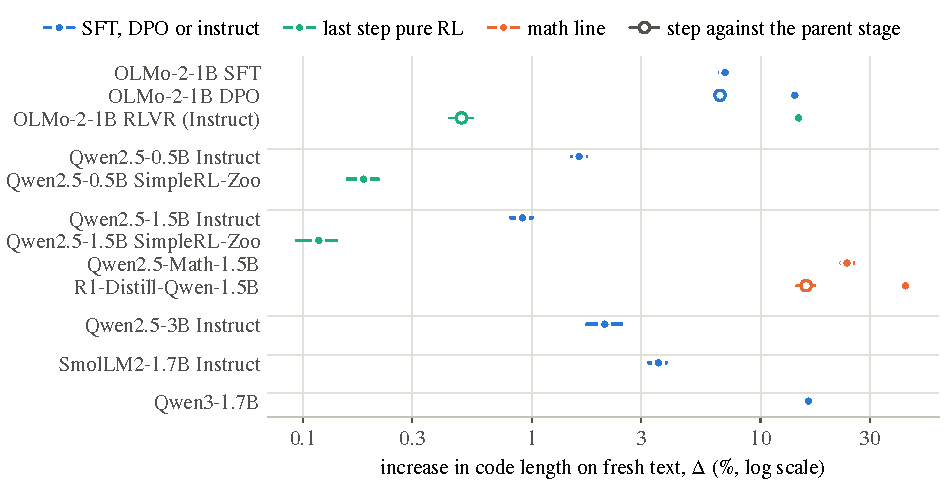
\includegraphics{figures/fig1_staged_drift.pdf}
\caption{Drift of each post-trained checkpoint on fresh text against its family base (filled), coloured by the
whole path from the base, and, for chained stages, against its parent stage (hollow), coloured by that step.
Lines are 95\% paired window-bootstrap intervals; some are narrower than the marker.}
\label{fig:stages}
\end{figure}

The increase spans more than two orders of magnitude. The two pure-RL checkpoints moved the code by 0.18\% and
0.12\%, 8.7 and 7.8 times less than the Instruct pipelines of the same sizes, and OLMo-2's RLVR step by 0.49\%,
fourteen times less than its SFT step; the amounts of training behind these steps differ and are not
normalised. The SFT
and DPO steps moved it by 1 to 7\%, and OLMo-2's DPO step ($+6.65\%$) was as large as its SFT step ($+6.99\%$),
against the 0 to 2\% expected. The largest increases belong to the mathematical line.

How the mathematical line divides between its two steps depends on the document-start convention. With the
end-of-text token, continued pretraining moved Qwen2.5-1.5B by 23.84\% and distillation added 15.81\%; with a
blank line as document start the two steps are 16.03\% and 20.90\%, so the division reverses while the total stays
near 40\% (40.21\%). The signs of the four laptop pairs survive the blank-line start ($+0.9$, $+4.1$, $+17.0$ and
$+20.9\%$ for Qwen2.5-1.5B, SmolLM2, Qwen3 and R1-Distill against Qwen2.5-Math), and restricting to tokens with at
least 128 tokens of context changes their deltas little. For Qwen3 and R1-Distill the worst 1\% of tokens carry 11
to 19\% of the extra bits, and the post-trained model is worse than its base on only 43 to 63\% of the tokens.

Against the family base the old control drifts 1.3 to 3.0 times as much as the fresh text. The two exceptions are
steps against a parent: RLVR against DPO (0.72) and R1-Distill against Qwen2.5-Math (0.62). The drift is not
specific to text written after the models were trained.

\subsection{One temperature recovers at most 35\%}
\label{sec:temperature}

If post-training only sharpened the predicted distributions, one temperature $T$ applied to the logits would
restore most of the code length. For the four laptop pairs we fitted $T^*$ on the even windows of each corpus and
measured on the odd windows (Table~\ref{tab:temperature}, Fig.~\ref{fig:temperature}). The rule, written down with
the results and not before them, called the increase mostly a confidence shift if both large-drift pairs recovered
at least 70\% and mostly a change of belief if both recovered at most 30\%.

\begin{table}[ht]
\centering\small
\caption{Temperature fit on the odd windows of the fresh corpora. Recovered is the share of the increase at $T=1$
removed by the post-trained model's own $T^*$ (mean of the three corpora, range over corpora in parentheses);
residual is the drift with each model at its own $T^*$.}
\label{tab:temperature}
\begin{tabular}{@{}l r c c r r@{}}
\toprule
Pair & $\Delta$ at $T=1$ & $T^*$ base & $T^*$ post & Recovered & Residual \\
\midrule
Qwen2.5-1.5B $\to$ Instruct & $+1.0\%$ & 1.00--1.05 & 1.00--1.06 & 15\% (1--42) & $+0.9\%$ \\
SmolLM2-1.7B $\to$ Instruct & $+3.7\%$ & 1.00--1.05 & 1.04--1.08 & 6\% (2--13) & $+3.6\%$ \\
Qwen3-1.7B-Base $\to$ Qwen3-1.7B & $+16.0\%$ & 1.00--1.04 & 1.22--1.28 & 35\% (31--39) & $+10.4\%$ \\
Qwen2.5-Math-1.5B $\to$ R1-Distill & $+15.4\%$ & 1.02--1.07 & 1.15--1.18 & 19\% (18--20) & $+12.7\%$ \\
\bottomrule
\end{tabular}
\end{table}

\begin{figure}[t]
\centering
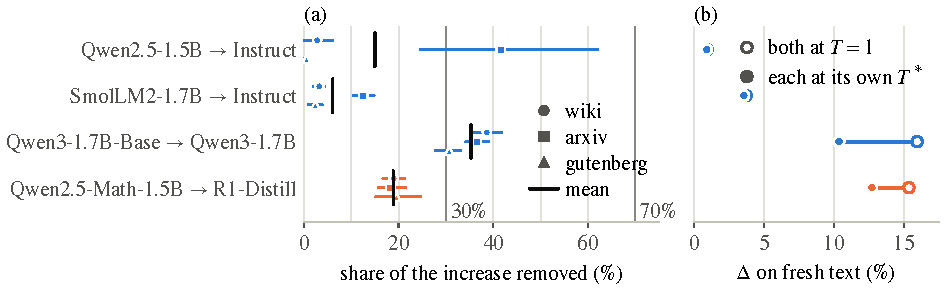
\includegraphics{figures/fig2_temperature.pdf}
\caption{(a) Share of the increase in code length removed by the post-trained model's own best temperature, per
fresh corpus, with 95\% window-bootstrap intervals; the black bar is the mean of the three corpora and the grey
lines are the rule's 30\% and 70\% boundaries. (b) Drift with both models at $T=1$ (hollow) and with each at its
own $T^*$ (filled), mean of the three fresh corpora.}
\label{fig:temperature}
\end{figure}

Qwen3 and R1-Distill are overconfident on this text: their best temperatures are about 1.25 and 1.16, while every
base model's lies between 0.995 and 1.07. Undoing the sharpening removes 35\% of Qwen3's increase (per-corpus
intervals 28 to 42\%) and 19\% of R1-Distill's, which leaves 10.4\% and 12.7\%; the two light instruction-tuned
pairs recover 6 and 15\%. Under the rule the verdict is mixed. One global temperature is the crudest calibrator,
and the recovered share does not by itself separate calibration from changed belief: Yang \citep{yang2026vocab}
found that a temperature with a vocabulary bias recovers 29\% of the loss increase even for weights perturbed at
random, and up to 36\% for instruction-tuned models on web text. Yang's mathematical models, continued
pretraining of Qwen2.5, recover 1.2 to 1.3\%; our 19\% is for the different step from Qwen2.5-Math to
R1-Distill, and we did not fit the continued-pretraining step itself.

\subsection{What the drift predicts on benchmarks}
\label{sec:benchmarks}

We benchmarked the 12 public checkpoints and their six bases (Table~\ref{tab:benchmarks},
Fig.~\ref{fig:benchmarks}). The pre-registered gate was a Pearson correlation of at least 0.8 between $\dfresh$
and forgetting over the 12. The pre-registered gain was the GSM8K gain without chat templates, whose correlation
with the drift had to stay below 0.3 in magnitude.

\begin{table}[ht]
\centering\small
\caption{The 12 public checkpoints. Forgetting $F$ in per cent of the base score with its floor, $F$ without the
two ARC tasks, the changes of ARC and MMLU accuracy in points, and the IFEval gain in points with each
post-trained model in its own chat template.}
\label{tab:benchmarks}
\begin{tabular}{@{}l r r r r r r r r@{}}
\toprule
Checkpoint & $\dfresh$ & $F$ & Floor & $F$ w/o ARC & ARC-e & ARC-c & MMLU & IFEval \\
\midrule
OLMo-2-1B SFT & $+6.99$ & $+0.01$ & 2.2 & $-2.03$ & $-3.6$ & $-1.3$ & $+5.9$ & $+31.5$ \\
OLMo-2-1B DPO & $+14.10$ & $-1.40$ & 2.2 & $-2.91$ & $-2.7$ & $+0.7$ & $+5.0$ & $+43.5$ \\
OLMo-2-1B RLVR & $+14.66$ & $-0.88$ & 2.2 & $-2.57$ & $-2.6$ & $-0.4$ & $+4.0$ & $+50.5$ \\
Qwen2.5-0.5B Instruct & $+1.61$ & $-0.22$ & 2.5 & $+0.51$ & $+0.5$ & $+1.3$ & $-2.2$ & $+13.0$ \\
Qwen2.5-0.5B SimpleRL & $+0.18$ & $-0.15$ & 2.5 & $+0.56$ & $+0.1$ & $+1.6$ & $-0.4$ & $+5.5$ \\
Qwen2.5-1.5B Instruct & $+0.91$ & $-1.78$ & 2.1 & $-0.36$ & $+4.4$ & $+1.4$ & $+0.5$ & $+18.0$ \\
Qwen2.5-1.5B SimpleRL & $+0.12$ & $-1.57$ & 2.1 & $+0.34$ & $+4.2$ & $+2.6$ & $+0.0$ & $-6.0$ \\
Qwen2.5-Math-1.5B & $+23.84$ & $+13.90$ & 2.1 & $+15.62$ & $-7.3$ & $-4.4$ & $-16.9$ & $+1.5$ \\
R1-Distill-Qwen-1.5B & $+42.95$ & $+21.61$ & 2.1 & $+21.34$ & $-15.5$ & $-10.4$ & $-23.3$ & $+5.5$ \\
Qwen2.5-3B Instruct & $+2.08$ & $-0.44$ & 1.9 & $-0.49$ & $-0.1$ & $+0.5$ & $-0.6$ & $+34.0$ \\
SmolLM2-1.7B Instruct & $+3.57$ & $+3.79$ & 2.1 & $-0.03$ & $-10.6$ & $-3.8$ & $-0.4$ & $+29.5$ \\
Qwen3-1.7B & $+16.18$ & $+4.67$ & 2.1 & $+6.41$ & $+1.3$ & $-2.1$ & $-5.9$ & $+46.5$ \\
\bottomrule
\end{tabular}
\end{table}

\begin{figure}[t]
\centering
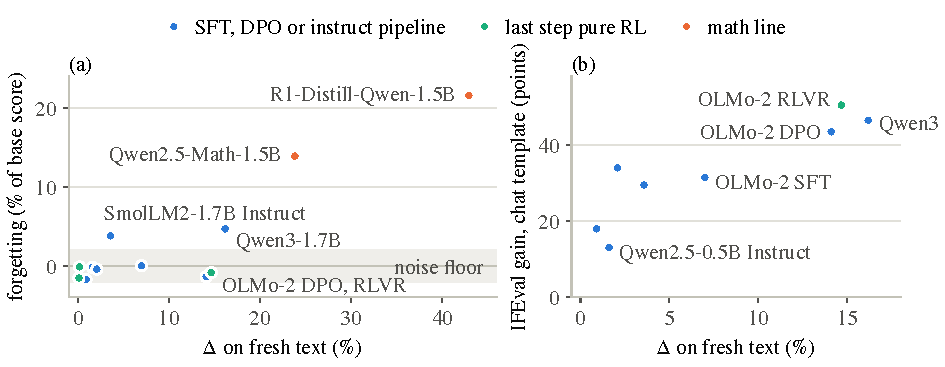
\includegraphics{figures/fig3_benchmarks.pdf}
\caption{(a) Forgetting against drift for the 12 public checkpoints; the grey band is the median noise floor,
$\pm2.1\%$ of the base score. (b) IFEval gain, each post-trained model in its own chat template, against drift
for the eight chat-tuned checkpoints (stages SFT, DPO, RLVR and instruct), a reading added after the main
result.}
\label{fig:benchmarks}
\end{figure}

The gate passes as written, $r=0.887$, and one lineage carries it. Qwen2.5-Math and R1-Distill drift by 24 and
43\% and lose 13.9 and 21.6\%; without them $r=0.32$ over the other ten. The 12 checkpoints form six families,
some of them chains, so they are not independent. Resampling families instead of checkpoints gives the interval
$[-0.64,\,0.99]$, and the correlation within families, each family's means removed, is 0.97, all of it from the
Qwen2.5-1.5B family. Under exchangeable checkpoints a one-sided permutation test gives $p=0.001$ for $r$ and
$p=0.01$ for Spearman's $\rho$ (0.67). With the blank-line document start for the five checkpoints scored that
way, $r=0.835$. The enwik8 drift gives $r=0.949$. Chance-adjusted forgetting, the aggregate form of the adjustment
of Harmon et al.\ \citep{harmon2025mapping}, ranks the 12 identically.

Read after the fact, the 12 points describe a threshold more than a ranking. Eight lie within their noise floor,
among them OLMo-2-DPO and -RLVR at 14.1 and 14.7\%, and the three above 15\% lie outside it: Qwen3 at 16.2\%
(forgetting 4.7\%), Qwen2.5-Math and R1-Distill. Any cut between 14.66 and 16.18\% describes these points equally
well, two of the three above it are one lineage, and of the eight checkpoints in this paper that forget beyond
the floor, a cut at 15\% contains three.

The per-task columns of Table~\ref{tab:benchmarks} show two kinds of loss. The mathematical line and Qwen3 lose
on several tasks, MMLU included, and keep most of their forgetting without ARC (15.6, 21.3 and 6.4\%).
SmolLM2-Instruct loses on ARC alone: without ARC its forgetting is $-0.03\%$. A six-task mean with no loss can hide
opposite movements. The OLMo-2 chain loses 2.6 to 3.6 points of ARC-Easy and gains 4.0 to 5.9 points of MMLU,
and without MMLU its forgetting is 1.9, 0.0 and 0.3\%; its DPO step doubles the drift and moves the six-task score
by nothing. The log-likelihood tasks were scored without chat templates, which the pre-registration had named as a
way for a change of format to look like forgetting.

The absolute code length still ranks the post-trained checkpoints. Across the six bases, fresh-text bpb and the
general score correlate at $r=-0.97$; across the 12 post-trained checkpoints at $r=-0.81$ ($\rho=-0.71$), and at
$-0.65$ without the mathematical line. Both quantities are likelihoods, scored on similar text, and the relation
says nothing of generation.

The drift is not a one-sided meter of loss. The pre-registered gain cannot be read for chat-tuned models:
prompted as a base model, SmolLM2-Instruct scores 0.0 on GSM8K, and the registered correlation ($r=+0.38$) mixes
format failures with gains. The chat-template condition was committed two minutes after the main result. With chat
templates the GSM8K gain is confounded by the 256-token cap (R1-Distill scores 15.7\%). IFEval, capped at 1,280
tokens, gives $r=0.89$ ($[0.70,\,0.99]$) over the eight chat-tuned checkpoints and $r=-0.03$ over all 12: OLMo-2 SFT,
DPO and RLVR at drifts of 7, 14 and 15\% gain 31.5, 43.5 and 50.5 points, and Qwen3 at 16\% gains 46.5. Across these
public checkpoints a larger drift went with a larger instruction-following gain.

\subsection{The token-class decomposition}
\label{sec:classes}

If the drift had one component on names, numbers and rare words that follows lost knowledge, and one on function
words and punctuation that follows changed style, the first might predict forgetting and the second the gain. The
pre-registered fail rule, a correlation above 0.9 between the two class drifts over the 12, triggered: $r=0.925$,
$[0.72,\,1.00]$. The trigger had been expected, for a reason that made it uninformative: the two mathematical
checkpoints drift far on every class, and without them $r=0.76$. Knowledge drift ranks the checkpoints exactly as
total drift does ($\rho=0.671$ for both), and both class drifts track the IFEval gain ($r=0.84$ and $0.81$), so
neither channel hypothesis passes. SmolLM2-Instruct puts 63.0\% [60.1, 66.2] of its extra bits on knowledge
tokens and OLMo-2-DPO 44.7\% [42.6, 46.8], as predicted, and knowledge tokens take more than their proportional
share in 9 of the 12 checkpoints. Lin et al.\ \citep{lin2023urial} found the shift from base to aligned model
concentrated on stylistic tokens; their measure is on the models' own responses, ours on independent text.

A secondary reading, registered without a threshold, gave a lead. The contrast \KS{} tracked forgetting at
$r=0.92$ over the 12 and $0.81$ $[0.41,\,0.98]$ without the mathematical line, where the total drift gave 0.32, and
did not track the IFEval gain ($r=0.17$, $n=8$). The lead was weak: without Qwen3 it falls to 0.55, and divided by
the total drift, a form free of the dose, it gives $r=0.24$ over the 12 and 0.45 without the mathematical line. Two
checkpoints carried it. OLMo-2-DPO drifts 14.1\% with a contrast of $-3.00$\pp{} and forgets nothing; Qwen3 drifts
16.2\% with $+14.12$\pp{} and forgets 4.7\%.

\subsection{The matched-recipe test}
\label{sec:matched}

The test held the base and the dose fixed and varied the recipe (Section~\ref{sec:recipes}). At a mark the three
recipes have nearly equal $\dfresh$: 3.02 to 3.28\% at the 3\% mark and 6.00 to 6.06\% at the 6\% mark.
Table~\ref{tab:matched} and Fig.~\ref{fig:matched} give the 12 checkpoints, with 95\% window-bootstrap intervals
for the contrast computed from the saved per-token bits.

\begin{table}[ht]
\centering\footnotesize
\caption{The 12 checkpoints of the controlled recipes. Passes over the 45M-token subset; contrast \KS{} with its
95\% window-bootstrap interval; forgetting $F$ in per cent of the base score, also without ARC; the changes of
ARC-Easy and MMLU accuracy in points (base 0.735 and 0.383); and the IFEval gain in points against the base in the
same template.}
\label{tab:matched}
\begin{tabular}{@{}l r l r r r c r r r r r@{}}
\toprule
Recipe & Update & Mark & Passes & $\dfresh$ & \multicolumn{2}{c}{\KS{} (pp) [95\%]} & $F$ & $F$ w/o ARC & ARC-e &
MMLU & IFEval \\
\midrule
\tulu & 1500 & final & 1.72 & $+2.02$ & $+1.69$ & [1.33, 2.04] & $-1.45$ & $-2.01$ & $-0.5$ & $+3.6$ & $+14.0$ \\
 & 1760 & 3\% & 2.02 & $+3.28$ & $+2.47$ & [2.00, 2.93] & $-0.30$ & $-2.05$ & $-2.8$ & $+5.6$ & $+15.5$ \\
 & 2660 & 6\% & 3.05 & $+6.01$ & $+3.37$ & [2.85, 3.88] & $-1.74$ & $-2.68$ & $-0.9$ & $+5.7$ & $+13.5$ \\
 & 3489 & final & 4.00 & $+7.11$ & $+4.35$ & [3.76, 4.92] & $-0.82$ & $-2.00$ & $-2.1$ & $+4.8$ & $+12.0$ \\
\smoltalk & 920 & 3\% & 1.02 & $+3.02$ & $+1.55$ & [1.04, 2.08] & $-0.97$ & $-1.94$ & $-1.4$ & $+4.4$ & $+10.5$ \\
 & 1500 & final & 1.67 & $+3.36$ & $+2.17$ & [1.65, 2.72] & $-0.83$ & $-1.81$ & $-1.8$ & $+4.9$ & $+13.0$ \\
 & 2500 & 6\% & 2.78 & $+6.00$ & $+2.38$ & [1.52, 3.27] & $-0.89$ & $-1.93$ & $-1.6$ & $+4.5$ & $+13.5$ \\
 & 3487 & final & 3.87 & $+8.97$ & $+3.41$ & [2.44, 4.41] & $-0.65$ & $-1.77$ & $-2.8$ & $+4.7$ & $+16.5$ \\
\mathcot & 1500 & final & 1.63 & $+2.50$ & $+2.10$ & [1.67, 2.53] & $+4.24$ & $+0.37$ & $-9.4$ & $-1.2$ & $+1.5$ \\
 & 1660 & 3\% & 1.81 & $+3.06$ & $+2.86$ & [2.42, 3.32] & $+4.07$ & $-0.04$ & $-9.7$ & $-0.8$ & $+3.0$ \\
 & 2780 & 6\% & 3.02 & $+6.06$ & $+3.41$ & [2.77, 4.09] & $+4.10$ & $+1.45$ & $-7.3$ & $-1.9$ & $+0.0$ \\
 & 3464 & final & 3.77 & $+7.14$ & $+4.48$ & [3.79, 5.21] & $+4.41$ & $+1.50$ & $-7.2$ & $-1.7$ & $+3.5$ \\
\bottomrule
\end{tabular}
\end{table}

\begin{figure}[t]
\centering
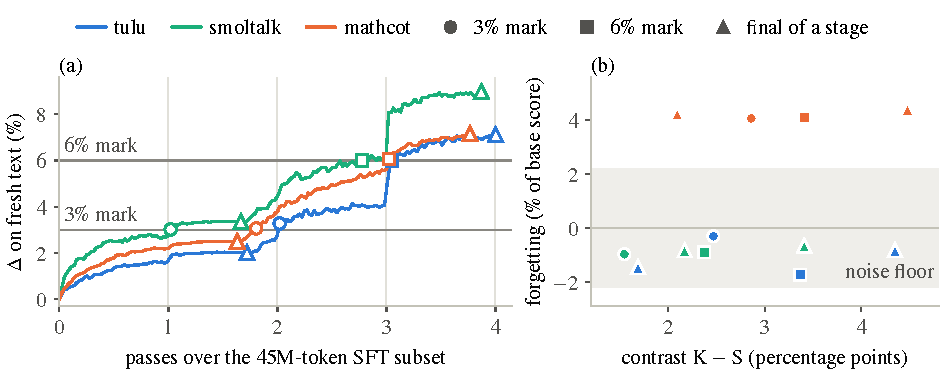
\includegraphics{figures/fig4_matched.pdf}
\caption{The controlled recipes on one base. (a) Drift on fresh text along each run against passes over the
training subset; markers are the benchmarked checkpoints, the first triangle of each run (1.6 to 1.7 passes) is
where the second stage restarted, and the jumps follow the pass boundaries. (b) Forgetting against the contrast
\KS{}, with 95\% window-bootstrap intervals; the grey band is the noise floor, $\pm2.2\%$ of the base score.}
\label{fig:matched}
\end{figure}

The pre-registered fail rule triggers, but the design could not have decided the test. Over the six marks
$r(K\!-\!S,\mathrm{forgetting})=0.43$, $[-0.79,\,1.00]$, below 0.6 (H1), and
$r(K\!-\!S,\mathrm{IFEval\ gain})=-0.41$, outside $\pm0.3$ (H2). The two could not both pass: across the 12
checkpoints forgetting and the IFEval gain correlate at $-0.94$ ($-0.93$ over the marks), as the expected values
registered beside the hypotheses had implied, so a perfect forgetting meter would also have failed H2. At the 6\%
mark the contrast orders the recipes \mathcot{} 3.41 $\approx$ \tulu{} 3.37 $>$ \smoltalk{} 2.38\pp, against the
predicted \mathcot{} $>$ \smoltalk{} $>$ \tulu{} (H4). The paired interval of \mathcot{} $-$ \tulu{} is
$[-0.58,\,0.74]$ at 6\% and $[-0.10,\,0.91]$ at 3\%, and with a seven-row median around each mark the order becomes
3.71 $>$ 3.37 $>$ 2.43 and holds. H4 is therefore undecided, and the trigger rests on H1 alone. The contrast does
separate \smoltalk{} from the other two: at 6\% \mathcot{} $-$ \smoltalk{} is 1.04 $[0.14,\,1.98]$ and \tulu{} $-$
\smoltalk{} 0.99 $[0.30,\,1.68]$. Over all 12 checkpoints H1 gives 0.29 and H2 $-0.20$, which passes. The contrast
grows with the dose within each recipe (pooled $r=0.80$ with $\dfresh$). The rare $-$ frequent variant gives
$r=0.69$ over the marks and 0.35 over all 12, and holds its predicted order by 0.06\pp.

Neither the drift nor the contrast tracked the outcomes. The drift correlates with forgetting at $r=-0.04$ and
with the IFEval gain at $r=0.13$ over the 12 ($-0.04$ over the marks). From the first checkpoint to the last the
drift of each recipe roughly triples while its forgetting and gain stay where they were: \tulu{} goes from 2.0 to 7.1\%
drift while its gain moves from 14.0 to 12.0 points, \mathcot{} from 2.5 to 7.1\% while its forgetting moves from
4.24 to 4.41\%. \mathcot{} forgets 4.07 to 4.41\% at every checkpoint, all of it on ARC: without ARC its forgetting
is $-0.04$ to $+1.50\%$, inside the floor, while ARC-Easy falls 7.2 to 9.7 points. \tulu{} and \smoltalk{} show no
loss on the six-task mean ($-1.74$ to $-0.30\%$), but they lose up to 2.8 points of ARC-Easy and gain 3.6 to 5.7
points of MMLU, and without MMLU their forgetting reaches 1.4 and 0.8\%. At matched drift the range of forgetting
across recipes is 5.0\pp{} at 3\% and 5.8\pp{} at 6\%, above the floor for the range of three checkpoints, about
2.6\pp{} (H3). The IFEval gain is also a property of the recipe: 12.0 to 15.5 points for \tulu{}, 10.5 to 16.5 for
\smoltalk{} and 0.0 to 3.5 for \mathcot{}, which was not trained for instruction following and whose mathematical
gain was not measured.

The drift also measures repetition. When a new pass over the training subset begins, the drift jumps within 20 to
40 updates while the training loss falls (Fig.~\ref{fig:matched}a): \tulu{} by 0.51\pp{} at its second pass and
1.64\pp{} at its third, \smoltalk{} by 0.27, 0.24 and 1.88\pp{} at its first three, and \mathcot{} by 0.50\pp{} at its
third, from 5.56 to 6.06\%, the jump that produced its 6\% mark. Four of the six marks were reached within 0.06
passes after a boundary, so matched drift was in part matched repetition. No checkpoint was evaluated immediately
on both sides of a jump. An exploratory reading of the drift's profile across corpora, stated before it was
computed but after the benchmarks were seen, failed its prediction; the forgetting recipe does drift least on
Wikipedia, at 0.70 and 0.82 of its fresh mean against 0.97 to 1.09 for the other two.

\section{Discussion}
\label{sec:discussion}

\subsection{Readings for practice}

For models of this size the measurements support three readings for practice. All three are conditional on a
further experiment that tests whether the ARC losses of \mathcot{} and SmolLM2-Instruct reflect answer format; if
they do, the readings concern the cloze format and not knowledge.
\begin{enumerate}
\item \emph{Benchmark the first saved checkpoint of a new recipe}, here the checkpoint after about one pass over
the data or at about 2\% drift. The loss of \mathcot{} was present at the first checkpoint evaluated (update
1,500, 1.6 passes, 2.5\% drift) and did not change over the following 1,964 updates. No earlier checkpoint was
evaluated, so the data do not say how early the loss appears, and the drift did not single out the recipe at any
dose.
\item \emph{Conversational SFT and DPO on these data left the six-task mean unchanged} up to a drift of 9\% in our
runs and 14.7\% in the OLMo-2 chain. The unchanged mean is a balance of ARC losses and MMLU gains, the floor
behind it favours a verdict of no change, and SmolLM2-Instruct, whose SFT data we reused on another base, lost
3.8\% on ARC at a drift of 3.6\%.
\item \emph{Read a large drift as a reason to benchmark, not as a verdict.} The public checkpoints that drift
above 15\% belong to two lineages, the Qwen2.5 mathematical line and Qwen3, and all three lost accuracy on several
tasks. This describes these points and is not a calibrated threshold: five of the eight forgetting checkpoints in
this paper lie below it.
\end{enumerate}
The drift is 11 to 37 times cheaper than the log-likelihood benchmarks, and it can be logged every few updates, as
we did every 20. It does not replace the first benchmark pass of a recipe.

The pass-boundary jumps suggest a use the experiments were not designed for. Each new pass over an SFT set raised
the drift by 0.1 to 1.9\pp{} within 40 updates, most at the third pass, together with a fall in training loss and
with no measured change in benchmarks, while between boundaries the drift moved slowly. Memorisation of training
data can be measured in bits \citep{morris2025memorize}, and a jump in fresh-text code length at a known
repetition would be a cheap online sign that a run has begun to memorise its SFT set. The sign is untested as a
detector: no checkpoint was evaluated on both sides of a jump, and it was seen in three runs on one base.

\subsection{Relation to prior work}

Our quantity is close to the forgetting measure of Kalajdzievski \citep{kalajdzievski2024scaling}, the
cross-entropy to the base model's predictions on WikiText-103; we evaluate it rather than propose it. Huang et
al.\ \citep{huang2024compression} excluded fine-tuned models from the relation between compression and benchmark
scores; for log-likelihood benchmarks the absolute code length of our post-trained checkpoints still follows it
($r=-0.81$), while the base-relative drift does not meter forgetting. Uncheatable Eval \citep{tan2026uncheatable}
scores fresh text for base models only, by design. Information Capacity \citep{yuan2025capacity} attributes
Qwen3's larger loss of compression to multi-stage RL, but Qwen3-1.7B was distilled \citep{yang2025qwen3}, and in
our checkpoints the RL steps moved the code length least. Yang \citep{yang2026vocab} measured the loss increase of
14 base and derived pairs on web text, two of them ours (Section~\ref{sec:temperature}). Shenfeld et al.\
\citep{shenfeld2025razor} found that the KL divergence from the base on the inputs of the new task predicts
forgetting; ours is measured on general text. Harmon et al.\ \citep{harmon2025mapping} report moderate forgetting
under domain-continual pretraining and low to moderate forgetting after RL or SFT from base models, as in our
mathematical line and SimpleRL checkpoints. Jin and Ren \citep{jin2024forgetting} predicted which upstream examples
a fine-tune forgets, and Marek et al.\ \citep{marek2026forgetting} showed that a KL penalty on pretraining or
self-generated text nearly removes forgetting; our results speak against the distance as a gauge at small doses,
not against it as a regulariser.

Several results bear on what our forgetting measures. Zheng et al.\ \citep{zheng2025spurious} found that drops in
continual learning often reflect a decline in task alignment rather than lost knowledge, one reading of losses
confined to ARC. Multiple-choice scores move with answer format and the method of answer selection
\citep{alzahrani2024benchmarks,zheng2024mcq}, which bears on the MMLU gains that offset ARC losses after SFT. The
alignment tax was reported for InstructGPT \citep{ouyang2022instructgpt}, which also chose its SFT learning rate
partly by a low loss on pretraining validation data, and Lin et al.\ \citep{lin2024alignmenttax} traced a Pareto
front between alignment and forgetting by averaging weights. Kostelec and Guo \citep{kostelec2026perplexity} showed
that log-likelihood scoring can understate a gap that appears in generation; our general benchmarks are scored by
log-likelihood.

\subsection{Limitations}

The conclusions hold within the following limits of the measurement.
\begin{enumerate}
\item All models have 0.5 to 3 billion parameters, and the controlled runs use one base, mid-trained on
instruction and mathematical data, and one seed.
\item The benchmarks are first-$N$ subsets, the floor is unpaired and covers item sampling only, and the
log-likelihood tasks were scored without chat templates.
\item The forgetting in the decisive cases is an ARC loss, and whether it reflects answer format is still under
test; the unchanged six-task means combine ARC losses with MMLU gains.
\item The 256-token generation cap was kept for GSM8K although it truncates long reasoning, so the gain of the
reasoning-trained checkpoints is unmeasured, and the IFEval gain of \mathcot{} is that of a recipe not trained for
it.
\item A recipe here bundles content, supervision density (25--27\% more supervised tokens for \mathcot{}), the
number of distinct examples and a length selection.
\item The second stage restarted the optimiser, its checkpoints were saved unannealed, and the marks were the
first crossings of a noisy series, four of them just after a pass boundary.
\item The public checkpoints number 12 in six families, the amount of training behind each stage is not
normalised, and the two leverage points are one continued-pretraining lineage.
\item The corpora are about 100\,KB each, two of the three are not all new writing, and the drift of the
mathematical line moves by 8 points with the document-start token.
\item The correlation tables of the experiments hold 148 pairs of Pearson and Spearman coefficients, with no
correction for multiplicity; the readings not registered in advance are marked as such.
\end{enumerate}
As the doses become smaller and the recipes more alike, the differences in forgetting become comparable with the
benchmark noise and depend more critically on the recipe, the benchmark format and the text that was scored.

\subsection{What would change the conclusions}

Six measurements would test these conclusions where they are weakest: a format control for the ARC losses
(letter-choice ARC, ARC in the chat template, or few-shot ARC), now running; the recipe test at 7 billion
parameters and with a second seed; full benchmarks with per-item outcomes, which allow paired tests; single-pass
recipes, which remove repetition from the dose; checkpoints before the first pass, which locate the onset of the
\mathcot{} loss; and a generation cap of 2,048 tokens or more, which measures the mathematical gain. A recipe whose
forgetting grew steadily with its drift, at fixed base, would overturn the reading of forgetting as a step.

\section{Summary}

We measured the increase in code length of post-trained language models on fresh text over their base models.
Post-training increased it at every stage, by about 0.1\% for pure RL, 1 to 7\% per step of SFT or DPO, and 16 to
43\% for distillation and mathematical training, and one temperature removes at most 35\% of the increase. Across
public checkpoints the increase went with the instruction-following gain and, above 15\% in two lineages, with lost
accuracy, readings made after the data were seen. Under recipe control it tracked neither: one recipe lost about
4\% on ARC from the first checkpoint evaluated, and the others lost nothing on a mean that balances ARC losses with
MMLU gains. The absolute code length still ranks post-trained models on log-likelihood benchmarks. As a cheap
signal of large departures, and perhaps of memorisation at repeated data, the drift is useful; as a meter of
forgetting at the doses of ordinary instruction tuning it is not.

\section*{Acknowledgements}

The experiments were implemented and executed with AI coding agents (Claude, by Anthropic) working under the
author's direction. The designs, pre-registrations and interpretations were reviewed by the author. Training and
benchmark runs used the GPU cluster of Aalborg University.

\bibliographystyle{plainnat}
\bibliography{refs}

\appendix

\section{Pre-registration and outcomes}
\label{app:prereg}

Table~\ref{tab:prereg} lists, for each experiment, the commit that registered its rules (times are CEST, 14--16
October 2026), every rule and expected value, the observed value, the verdict, and the deviations from the plan.
For experiments 3 to 6 the registered text is unchanged in the results commit.

{\footnotesize
\setlength{\LTpre}{0.5ex}\setlength{\LTpost}{0pt}
\begin{longtable}{@{}>{\raggedright\arraybackslash}p{0.04\textwidth} >{\raggedright\arraybackslash}p{0.42\textwidth}
>{\raggedright\arraybackslash}p{0.34\textwidth} >{\raggedright\arraybackslash}p{0.14\textwidth}@{}}
\caption{Registration, rules and expectations against the outcomes, and the deviations from each plan.}
\label{tab:prereg}\\
\toprule
Exp. & Rule or expectation & Observed & Verdict \\
\midrule
\endfirsthead
\toprule
Exp. & Rule or expectation & Observed & Verdict \\
\midrule
\endhead
\bottomrule
\endfoot
1 & \multicolumn{3}{>{\raggedright\arraybackslash}p{0.92\textwidth}@{}}{\emph{Not registered}; code and results in
2d9c318. All 12 pair and corpus drifts are positive with intervals above zero. \emph{Deviations from the plan:} a
document-start token is scored before every window; the planned news corpus was replaced by Gutenberg, because
Wikinews has published nothing since May 2026.} \\
\addlinespace
2 & \multicolumn{3}{>{\raggedright\arraybackslash}p{0.92\textwidth}@{}}{\emph{Rule committed with the results}
(762d4da, 20:05, 14 Oct), so not verifiable as registered; Yang's ``at most 36\%'' was already in the project notes
(c140ced, 19:31).} \\
 & Both large-drift pairs recover $\geq70\%$: confidence shift; both $\leq30\%$: change of belief; else mixed &
Qwen3 35\%, R1-Distill 19\% & mixed \\
 & \multicolumn{3}{>{\raggedright\arraybackslash}p{0.92\textwidth}@{}}{\emph{Deviations.} The check of $T=1$
against experiment 1 failed for four rows from a superseded fp16 conversion; rescoring matched to
$1.1\times10^{-6}$.} \\
\addlinespace
3 & \multicolumn{3}{>{\raggedright\arraybackslash}p{0.92\textwidth}@{}}{\emph{Registered} in 9562f71 (20:21, 14
Oct); the job started at 20:23; results c94d9a5 (20:46).} \\
 & E1: OLMo-2 SFT step $+3$ to $+8\%$ and the largest; E2: DPO step $+0$ to $+2\%$; E3: RLVR step within
$\pm1\%$; E4, E5: SimpleRL-Zoo $+0.5$ to $+3\%$ & $+6.99\%$ (largest by 0.34); $+6.65\%$; $+0.49\%$; $+0.18$ and
$+0.12\%$ & met narrowly; not met; met; not met \\
 & Headline: an RL stage below its predecessor with its interval below zero & none on any corpus & not triggered \\
 & Reproduction of the four laptop models within $10^{-3}$\,bpb & within $5\times10^{-5}$ & met \\
\addlinespace
4 & \multicolumn{3}{>{\raggedright\arraybackslash}p{0.92\textwidth}@{}}{\emph{Registered} in abc08d9 and f33fa18
(21:01--21:02, 14 Oct), decoding notes 9f22ff0 (22:00); array 22:20--23:58; results 669d2bc (00:02, 15 Oct).} \\
 & Gate 1: $r(\dfresh,\mathrm{forgetting})\geq0.8$ pass, $\geq0.6$ soft & $0.887$; family bootstrap $[-0.64,
0.99]$ & pass, on one lineage \\
 & One-sidedness: $|r(\dfresh,\mathrm{GSM8K\ gain})|<0.3$ & $+0.383$ & not shown \\
 & E1: $0.6\leq r<0.8$; E2: $r$ with the gain below 0.3 & 0.887; $+0.383$ & not met; not met \\
 & E3: enwik8 $r\geq$ fresh $r-0.05$; E4: R1-Distill has the largest drift and lies below the line & 0.949 against
0.887; largest, 2.1 points above & met; not met \\
 & \multicolumn{3}{>{\raggedright\arraybackslash}p{0.92\textwidth}@{}}{\emph{Deviations and later readings.} The
chat-template gain was committed after the main result (c295d52, 00:04) and became the primary gain measure; the
threshold reading was added after the run, and the Spearman and leave-one-out readings after an interim look; the chat-tuned subset has 8
checkpoints, not the 9 stated; sample-wise forgetting was not computed because samples were not logged.} \\
\addlinespace
5 & \multicolumn{3}{>{\raggedright\arraybackslash}p{0.92\textwidth}@{}}{\emph{Registered} with the analysis code
in 1eb436a (14:46, 15 Oct), before any class drift existed; results e689078 (15:01).} \\
 & Fail rule: $r(\Delta_K,\Delta_S)>0.9$ over the 12 & 0.925 (0.76 without the math line) & triggered \\
 & H1: knowledge drift ranks forgetting at least as well as total drift, and $r\geq0.6$ without the math line &
$\rho$ 0.671 against 0.671; $r=0.48$ & fail \\
 & H2: $r(\Delta_S,\mathrm{gain})\geq0.8$ and $r(\Delta_K,\mathrm{gain})<0.5$ & 0.805 and 0.844 & fail \\
 & H3: knowledge share of SmolLM2-Instruct above OLMo-2-DPO's; H4: $\rho$(enwik8 excess, MMLU loss)
$\geq\rho(\dfresh$, MMLU loss); E1: the fail rule triggers; E2: class order of four checkpoints & 63.0 [60.1,
66.2] against 44.7 [42.6, 46.8]; 0.42 against 0.34; both as predicted & pass; pass, weak; met \\
 & \multicolumn{3}{>{\raggedright\arraybackslash}p{0.92\textwidth}@{}}{\emph{Deviations.} Tagger artefacts were
left uncorrected (LaTeX mathematics tagged as proper nouns, hyphen-led pieces as punctuation); the frequency-only
variant, free of both, gives the same verdicts.} \\
\addlinespace
6 & \multicolumn{3}{>{\raggedright\arraybackslash}p{0.92\textwidth}@{}}{\emph{Registered} in 9cca20f (15:24, 15
Oct), before any training step; deviations becc72a (16:36) and 0454f34 (20:39), each before the runs they affect;
the exploratory hypothesis ec2e6f6 (08:22, 16 Oct); results c0944b1 (08:28).} \\
 & H1: $r(K\!-\!S,\mathrm{forgetting})\geq0.8$ pass, $\geq0.6$ soft, over the marks & 0.431 (0.29 over all 12) &
fail \\
 & H2: $|r(K\!-\!S,\mathrm{IFEval\ gain})|<0.3$ & $-0.405$ ($-0.20$ over all 12) & fail (pass) \\
 & H3: forgetting range across recipes above the floor at $\geq2$ marks & 5.04 and 5.83 against 2.22\pp{} (2.65
for a range of three) & pass \\
 & H4: contrast and forgetting ordered \mathcot{} $>$ \smoltalk{} $>$ \tulu{} at 6\% & contrast 3.41, 2.38, 3.37;
\mathcot{} $-$ \tulu{} $[-0.58, 0.74]$ & fail as registered; undecided \\
 & Fail rule: $r(K\!-\!S,\dfresh)>0.9$, or H1 $<0.6$ with the H4 order violated & H1 0.43, order violated within
noise & triggered \\
 & E0: every recipe reaches 6\% within 1,500 updates & none did & not met \\
 & E1: H1 at least soft and H2 pass; E2: the fail rule does not trigger & neither; H1 and H2 incompatible given
$r(F,\mathrm{gain})=-0.94$ & not met \\
 & At 6\% for \tulu{}, \smoltalk{}, \mathcot{}: forgetting $0\pm2$, 2 to 4, 3 to 8; contrast $-3$ to $+1$, $+2$ to
$+5$, $+5$ to $+12$; IFEval gain in that order & $-1.74$, $-0.89$, $+4.10$; $+3.37$, $+2.38$, $+3.41$; 13.5, 13.5,
0.0 & met, not, met; not, met, not; tie, then met \\
 & \multicolumn{3}{>{\raggedright\arraybackslash}p{0.92\textwidth}@{}}{\emph{Deviations.} The wall-time cap was
raised from 5 to 8.5 hours after the dry run measured 15.4\,s per update; the second stage was registered before
any of its updates; 1,500 updates gave 1.6--1.7 passes, not the 2.2 planned, because of padding; the 10\% mark was
never reached, so H3 was scored on two marks and H1 and H2 on six checkpoints, not nine; the per-corpus hypothesis
was stated after the benchmarks were seen and was not supported.} \\
\end{longtable}
}

\section{Compute, software, models and reproduction}
\label{app:compute}

The cluster work totals about 59 GPU-hours, excluding dry runs (Table~\ref{tab:compute}).

\begin{table}[ht]
\centering\footnotesize
\caption{Compute per experiment.}
\label{tab:compute}
\begin{tabularx}{\textwidth}{@{}l l X@{}}
\toprule
Experiment & Hardware & Compute \\
\midrule
1, raw and chat scoring & Apple M2 Pro, MPS, fp16 & 21 min for the main table, 11 min for the document-start ablation \\
2, temperature & Apple M2 Pro, MPS, fp16 & 25 min of scoring \\
3, staged checkpoints & 1 Tesla T4, fp16 & 18 min 42 s for 14 models and 4 corpora (0.3 GPU-hours) \\
4, benchmarks & NVIDIA A10 & 6.2 GPU-hours for 18 checkpoints; 3.3 for the chat-template addendum \\
5, token classes & Apple M2 Pro, CPU & 68 s, no new scoring \\
6, controlled recipes & NVIDIA A40 and A10 & about 45 A40-hours of training, about 4 A10-hours of evaluation, 29 min of CPU \\
\bottomrule
\end{tabularx}
\end{table}

\emph{Software.} Python 3.12. On the laptop: PyTorch 2.14.1, transformers 5.19.0, NumPy 2.5.4, pandas 3.0.6 and
Matplotlib 3.11.2. On the cluster: the NGC PyTorch 25.09 container (PyTorch 2.9.0a0), transformers 5.19.0,
lm-evaluation-harness 0.4.13, datasets 5.1.0 and accelerate 1.15.0. For the token classes: spaCy 3.8.16 with
\texttt{en\_core\_web\_sm} 3.8.0 and wordfreq 3.1.1. The SFT datasets were loaded at the revisions recorded in
their provenance files: T\"ulu 3 SFT mixture \texttt{b14afda}, SmolTalk \texttt{5feaf2f}, OpenR1-Math-220k
\texttt{e4e141e}.

\emph{Model revisions.} The runs loaded each model's \texttt{main} revision and the cluster runs did not record
it. The laptop's Hugging Face cache, which experiments 1, 2 and 5 used, holds the snapshots below (first seven hex
digits of the commit); experiment 1's download log records the same snapshot for each of its nine models. The
cluster runs of 14--16 October 2026 loaded the revisions current on those dates.

{\footnotesize\sloppy\noindent
OLMo-2-0425-1B \texttt{a1847df}, -SFT \texttt{0d85a3d}, -DPO \texttt{c4b0485}, -Instruct \texttt{48d788e};
Qwen2.5-0.5B \texttt{060db64}, -Instruct \texttt{7ae5576}; Qwen-2.5-0.5B-SimpleRL-Zoo \texttt{e89bce4};
Qwen2.5-1.5B \texttt{8faed76}, -Instruct \texttt{989aa79}; Qwen-2.5-1.5B-SimpleRL-Zoo \texttt{c014eda};
Qwen2.5-Math-1.5B \texttt{4a83ca6}; DeepSeek-R1-Distill-Qwen-1.5B \texttt{ad9f0ae}; Qwen2.5-3B \texttt{3aab1f1},
-Instruct \texttt{aa8e725}; SmolLM2-1.7B \texttt{effd688}, -Instruct \texttt{31b70e2}; Qwen3-1.7B-Base
\texttt{ea980cb}; Qwen3-1.7B \texttt{70d244c}.\par}

\emph{Repository and reproduction.} The code, the dated corpora with their provenance files, the per-token bits,
the benchmark summaries and this report are public at \url{https://github.com/gottn/compression-intelligence}.
Experiments 3, 4 and 6 ran on a Slurm cluster through the job files in \texttt{infra/}; each experiment is rerun
with \texttt{bash expNN\_*/run\_all.sh}, whose header lists the steps. Per-item benchmark outputs were not logged
and the checkpoints of experiment 6 are not released. \texttt{make -C paper} recomputes the derived numbers
(\texttt{paper/derived.py}) and the figures (\texttt{paper/figures/make\_figures.py}, which checks every plotted
number against the experiments' RESULTS.md) and rebuilds this report; \texttt{./check.sh} runs the linter and the
tests.

\end{document}
